\subsection{Using a Language Model During Training}
\label{sec:trainwithlm}

A PT contains significant information beyond any single
transcript extracted from the PT. Motivated by this, the statistics
for ASR adaptation are accumulated from a lattice derived from the
cascade $H\circ C \circ PT$, rather than reducing the PT to its single
best path. Though it is disadvantageous to reduce a PT to its best
path, it is nevertheless advantageous to incorporate as much
information as possible about the target language during adaptation.
Define $G$ to be an FST representing the modeled phone bigram
probability
$\pi(\phi^\ell|\theta)=\prod_{m=1}^M\pi(\phi_m^\ell|\phi_{m-1}^\ell,\theta)$.
Training results can be improved by using $H\circ C\circ PT\circ G$ to
compute segmental K-means.

\begin{figure}
  \centerline{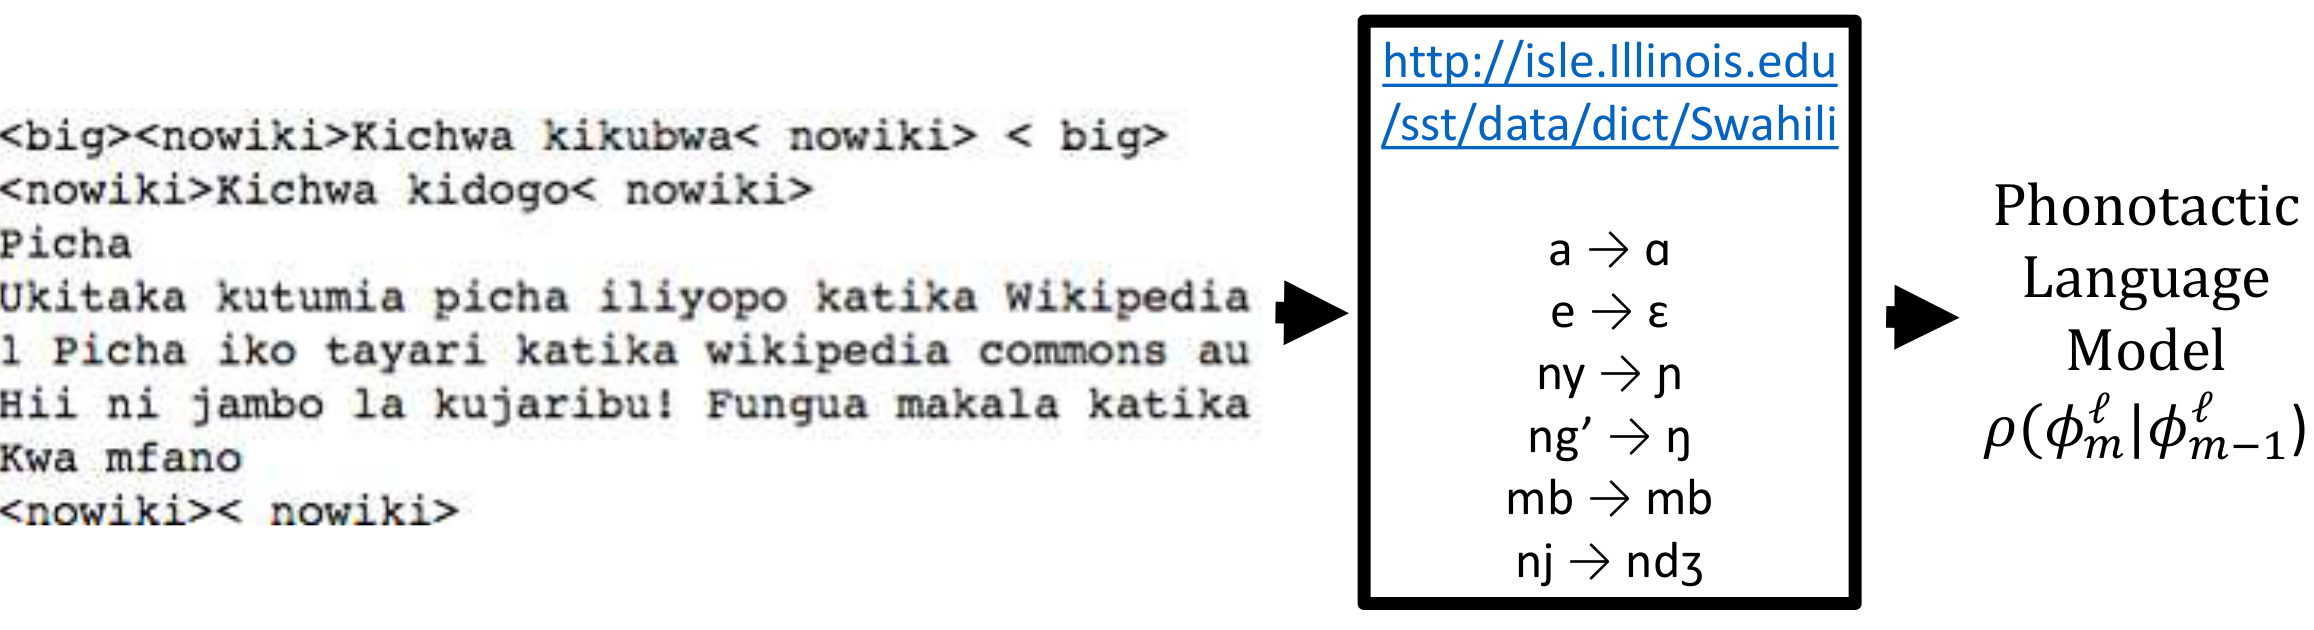
\includegraphics[width=0.8\columnwidth]{../figs/fig_sloan.png}}
  \vspace*{-3mm}
  \caption{A phonotactic language model (a bigram language model over
    phone sequences) can be trained using text data downloaded from
    Wikipedia (left), then converted into phone strings in the target
    language using a simple character-based grapheme-to-phoneme
    transducer (center).  In this example, the target language is
    Swahili.}
  \label{fig:wikitext}
\end{figure}

By assumption, phone bigram information is not available from speech:
we assume that there is no transcribed speech in the target language.
A reasonable proxy, however, can be constructed from text.
Fig.~\ref{fig:wikitext} shows text data downloaded from Wikipedia in
Swahili, and a segment of a rule-based, character-by-character G2P for
the Swahili language~\cite{Hasegawajohnson15}.  By passing the former
through the latter, it is possible to generate synthetic phoneme
sequences in the target language.

Composing $PT\circ G$ is complicated by the presence of null
transitions in the PT.  A null transition in the PT matches a
non-event in the language model, for which normal FST notation has no
representation. In order to compose the PT with the language model,
therefore, it is necessary to introduce a special type of
``non-event'' symbol, here denoted ``\#2'', into the language model
(Fig.~\ref{fig:liu1}).  As shown in Fig.~\ref{fig:liu1}, a language
model ``non-event'' is a transition that leaves any state, and returns
to the same state (a self-loop).  Such self-loops, labeled with the
special symbol ``\#2'' on both input and output language, are added to
every state in the phonotactic language model (left-hand side of
Fig.~\ref{fig:liu1}).  The probabilistic transcript, then, is
augmented with the special symbol ``\#2'' as the input-language symbol
for every null-output edge (output symbol is $\phi_m^\ell =\emptyset$).
\begin{figure}
\begin{center}
  \tikzstyle{pre}=[<-,shorten <=1pt,>=stealth',semithick,draw=black]
  \tikzstyle{post}=[->,shorten >=1pt,>=stealth',semithick,draw=black]
  \begin{tikzpicture}[
      scale=\mytikzscale,
      state/.style={circle,thick, draw=black, text=black, text width=0.25cm},
      compose/.style={circle,thick, draw=black, text=black, text width=0.1cm},
      every node/.style={transform shape}
    ]
    \node[state] (g0) at (-1.5,1) {};
    \node[state] (g1) at (1.5,1) {};
    \node[state] (g2) at (0,-1) {};
    \draw[post] (g0) -- (-1.75,1.5) -- (-1.5,1.75) -- (-1.25,1.5) -- (g0);
    \draw[post] (g0) -- (-2,0.75) -- (-2.25,1) -- (-2,1.25) -- (g0);
    \draw[post] (g1) -- (1.25,1.5) -- (1.5,1.75) -- (1.75,1.5) -- (g1);
    \draw[post] (g1) -- (2,1.25) -- (2.25,1) -- (2,0.75) -- (g1);
    \draw[post] (g2) -- (0.25,-1.5) -- (0,-1.75) -- (-0.25,-1.5) -- (g2);
    \draw[post] (g0) -- (g1);
    \draw[pre] (g0) -- (g2);
    \draw[pre] (g2) -- (g1);
    \draw[pre] (g0) -- (-1,1.5) -- (1,1.5) -- (g1);
    \draw[post] (g0) -- (-1.65,0.2) -- (-0.75,-1) -- (g2);
    \draw[post] (g2) -- (0.75,-1) -- (1.65,0.2) -- (g1);
    \node at (0,1.75) {a:a$/p(a|b)$};
    \node at (0,0.75) {b:b$/p(b|a)$};
    \node at (-3.25,1) {a:a$/p(a|a)$};
    \node at (3.25,1) {b:b$/p(b|b)$};
    \node at (-2,-0.5) {\#0:$\epsilon$$/\beta(a)$};
    \node at (-0.45,0.1) {a:a};
    \node at (2,-0.5) {b:b$/p(b)$};
    \node at (0.4,0.15) {\#0:$\epsilon$};
    \node at (-1.5,2) {\#2:\#2};
    \node at (1.5,2) {\#2:\#2};
    \node at (0,-2) {\#2:\#2};
    \node[compose] (c) at (4,0) {};
    \node[state] (pt0) at (6,0) {};
    \node[state] (pt1) at (8,0) {};
    \node[state] (pt2) at (10,0) {};
    \node[compose] (pt2inner) at (10,0) {};
    \draw[post] (pt0) -- (6.5,0.5) -- (7.5,0.5) -- (pt1);
    \draw[post] (pt0) -- (6.5,-0.5) -- (7.5,-0.5) -- (pt1);
    \draw[post] (pt1) -- (8.5,0.5) -- (9.5,0.5) -- (pt2);
    \draw[post] (pt1) -- (8.5,-0.5) -- (9.5,-0.5) -- (pt2);
    \node at (7,0.75) {a:a$/0.8$};
    \node at (7,-0.75) {\#2:$\emptyset$$/0.2$};
    \node at (9,0.75) {b:b$/0.8$};
    \node at (9,-0.75) {a:a$/0.2$};
  \end{tikzpicture}
\end{center}
\vspace*{-2mm}
\caption{Deletion edges in the probabilistic transcript (edges with
  the special null-phone symbol, $\emptyset$), required special
  handling in order to use information from a phonotactic language
  model.  As shown, a new type of null symbol, ``\#2'', was invented
  to represent the input for every PT edge with an $\emptyset$ output
  (right).  Such edges were only allowed to match with state
  self-loops, newly added to the language model (left) in order to
  consume such non-events in the transcript.  a,b: regular phone
  symbols, $\epsilon$: null-string, $p(b|a)$: bigram probability,
  $\beta(a)$: language model backoff.}
\label{fig:liu1}
\end{figure}

